% Options for packages loaded elsewhere
\PassOptionsToPackage{unicode}{hyperref}
\PassOptionsToPackage{hyphens}{url}
\PassOptionsToPackage{dvipsnames,svgnames,x11names}{xcolor}
%
\documentclass[
]{ccr}

\usepackage{amsmath,amssymb}
\usepackage{lmodern}
\usepackage{iftex}
\ifPDFTeX
  \usepackage[T1]{fontenc}
  \usepackage[utf8]{inputenc}
  \usepackage{textcomp} % provide euro and other symbols
\else % if luatex or xetex
  \usepackage{unicode-math}
  \defaultfontfeatures{Scale=MatchLowercase}
  \defaultfontfeatures[\rmfamily]{Ligatures=TeX,Scale=1}
\fi
% Use upquote if available, for straight quotes in verbatim environments
\IfFileExists{upquote.sty}{\usepackage{upquote}}{}
\IfFileExists{microtype.sty}{% use microtype if available
  \usepackage[]{microtype}
  \UseMicrotypeSet[protrusion]{basicmath} % disable protrusion for tt fonts
}{}
\makeatletter
\@ifundefined{KOMAClassName}{% if non-KOMA class
  \IfFileExists{parskip.sty}{%
    \usepackage{parskip}
  }{% else
    \setlength{\parindent}{0pt}
    \setlength{\parskip}{6pt plus 2pt minus 1pt}}
}{% if KOMA class
  \KOMAoptions{parskip=half}}
\makeatother
\usepackage{xcolor}
\setlength{\emergencystretch}{3em} % prevent overfull lines
\setcounter{secnumdepth}{-\maxdimen} % remove section numbering
% Make \paragraph and \subparagraph free-standing
\ifx\paragraph\undefined\else
  \let\oldparagraph\paragraph
  \renewcommand{\paragraph}[1]{\oldparagraph{#1}\mbox{}}
\fi
\ifx\subparagraph\undefined\else
  \let\oldsubparagraph\subparagraph
  \renewcommand{\subparagraph}[1]{\oldsubparagraph{#1}\mbox{}}
\fi

\usepackage{color}
\usepackage{fancyvrb}
\newcommand{\VerbBar}{|}
\newcommand{\VERB}{\Verb[commandchars=\\\{\}]}
\DefineVerbatimEnvironment{Highlighting}{Verbatim}{commandchars=\\\{\}}
% Add ',fontsize=\small' for more characters per line
\usepackage{framed}
\definecolor{shadecolor}{RGB}{241,243,245}
\newenvironment{Shaded}{\begin{snugshade}}{\end{snugshade}}
\newcommand{\AlertTok}[1]{\textcolor[rgb]{0.68,0.00,0.00}{#1}}
\newcommand{\AnnotationTok}[1]{\textcolor[rgb]{0.37,0.37,0.37}{#1}}
\newcommand{\AttributeTok}[1]{\textcolor[rgb]{0.40,0.45,0.13}{#1}}
\newcommand{\BaseNTok}[1]{\textcolor[rgb]{0.68,0.00,0.00}{#1}}
\newcommand{\BuiltInTok}[1]{\textcolor[rgb]{0.00,0.23,0.31}{#1}}
\newcommand{\CharTok}[1]{\textcolor[rgb]{0.13,0.47,0.30}{#1}}
\newcommand{\CommentTok}[1]{\textcolor[rgb]{0.37,0.37,0.37}{#1}}
\newcommand{\CommentVarTok}[1]{\textcolor[rgb]{0.37,0.37,0.37}{\textit{#1}}}
\newcommand{\ConstantTok}[1]{\textcolor[rgb]{0.56,0.35,0.01}{#1}}
\newcommand{\ControlFlowTok}[1]{\textcolor[rgb]{0.00,0.23,0.31}{#1}}
\newcommand{\DataTypeTok}[1]{\textcolor[rgb]{0.68,0.00,0.00}{#1}}
\newcommand{\DecValTok}[1]{\textcolor[rgb]{0.68,0.00,0.00}{#1}}
\newcommand{\DocumentationTok}[1]{\textcolor[rgb]{0.37,0.37,0.37}{\textit{#1}}}
\newcommand{\ErrorTok}[1]{\textcolor[rgb]{0.68,0.00,0.00}{#1}}
\newcommand{\ExtensionTok}[1]{\textcolor[rgb]{0.00,0.23,0.31}{#1}}
\newcommand{\FloatTok}[1]{\textcolor[rgb]{0.68,0.00,0.00}{#1}}
\newcommand{\FunctionTok}[1]{\textcolor[rgb]{0.28,0.35,0.67}{#1}}
\newcommand{\ImportTok}[1]{\textcolor[rgb]{0.00,0.46,0.62}{#1}}
\newcommand{\InformationTok}[1]{\textcolor[rgb]{0.37,0.37,0.37}{#1}}
\newcommand{\KeywordTok}[1]{\textcolor[rgb]{0.00,0.23,0.31}{#1}}
\newcommand{\NormalTok}[1]{\textcolor[rgb]{0.00,0.23,0.31}{#1}}
\newcommand{\OperatorTok}[1]{\textcolor[rgb]{0.37,0.37,0.37}{#1}}
\newcommand{\OtherTok}[1]{\textcolor[rgb]{0.00,0.23,0.31}{#1}}
\newcommand{\PreprocessorTok}[1]{\textcolor[rgb]{0.68,0.00,0.00}{#1}}
\newcommand{\RegionMarkerTok}[1]{\textcolor[rgb]{0.00,0.23,0.31}{#1}}
\newcommand{\SpecialCharTok}[1]{\textcolor[rgb]{0.37,0.37,0.37}{#1}}
\newcommand{\SpecialStringTok}[1]{\textcolor[rgb]{0.13,0.47,0.30}{#1}}
\newcommand{\StringTok}[1]{\textcolor[rgb]{0.13,0.47,0.30}{#1}}
\newcommand{\VariableTok}[1]{\textcolor[rgb]{0.07,0.07,0.07}{#1}}
\newcommand{\VerbatimStringTok}[1]{\textcolor[rgb]{0.13,0.47,0.30}{#1}}
\newcommand{\WarningTok}[1]{\textcolor[rgb]{0.37,0.37,0.37}{\textit{#1}}}

\providecommand{\tightlist}{%
  \setlength{\itemsep}{0pt}\setlength{\parskip}{0pt}}\usepackage{longtable,booktabs,array}
\usepackage{calc} % for calculating minipage widths
% Correct order of tables after \paragraph or \subparagraph
\usepackage{etoolbox}
\makeatletter
\patchcmd\longtable{\par}{\if@noskipsec\mbox{}\fi\par}{}{}
\makeatother
% Allow footnotes in longtable head/foot
\IfFileExists{footnotehyper.sty}{\usepackage{footnotehyper}}{\usepackage{footnote}}
\makesavenoteenv{longtable}
\usepackage{graphicx}
\makeatletter
\def\maxwidth{\ifdim\Gin@nat@width>\linewidth\linewidth\else\Gin@nat@width\fi}
\def\maxheight{\ifdim\Gin@nat@height>\textheight\textheight\else\Gin@nat@height\fi}
\makeatother
% Scale images if necessary, so that they will not overflow the page
% margins by default, and it is still possible to overwrite the defaults
% using explicit options in \includegraphics[width, height, ...]{}
\setkeys{Gin}{width=\maxwidth,height=\maxheight,keepaspectratio}
% Set default figure placement to htbp
\makeatletter
\def\fps@figure{htbp}
\makeatother
\newlength{\cslhangindent}
\setlength{\cslhangindent}{1.5em}
\newlength{\csllabelwidth}
\setlength{\csllabelwidth}{3em}
\newlength{\cslentryspacingunit} % times entry-spacing
\setlength{\cslentryspacingunit}{\parskip}
\newenvironment{CSLReferences}[2] % #1 hanging-ident, #2 entry spacing
 {% don't indent paragraphs
  \setlength{\parindent}{0pt}
  % turn on hanging indent if param 1 is 1
  \ifodd #1
  \let\oldpar\par
  \def\par{\hangindent=\cslhangindent\oldpar}
  \fi
  % set entry spacing
  \setlength{\parskip}{#2\cslentryspacingunit}
 }%
 {}
\usepackage{calc}
\newcommand{\CSLBlock}[1]{#1\hfill\break}
\newcommand{\CSLLeftMargin}[1]{\parbox[t]{\csllabelwidth}{#1}}
\newcommand{\CSLRightInline}[1]{\parbox[t]{\linewidth - \csllabelwidth}{#1}\break}
\newcommand{\CSLIndent}[1]{\hspace{\cslhangindent}#1}

\makeatletter
\makeatother
\makeatletter
\makeatother
\makeatletter
\@ifpackageloaded{caption}{}{\usepackage{caption}}
\AtBeginDocument{%
\ifdefined\contentsname
  \renewcommand*\contentsname{Table of contents}
\else
  \newcommand\contentsname{Table of contents}
\fi
\ifdefined\listfigurename
  \renewcommand*\listfigurename{List of Figures}
\else
  \newcommand\listfigurename{List of Figures}
\fi
\ifdefined\listtablename
  \renewcommand*\listtablename{List of Tables}
\else
  \newcommand\listtablename{List of Tables}
\fi
\ifdefined\figurename
  \renewcommand*\figurename{Figure}
\else
  \newcommand\figurename{Figure}
\fi
\ifdefined\tablename
  \renewcommand*\tablename{Table}
\else
  \newcommand\tablename{Table}
\fi
}
\@ifpackageloaded{float}{}{\usepackage{float}}
\floatstyle{ruled}
\@ifundefined{c@chapter}{\newfloat{codelisting}{h}{lop}}{\newfloat{codelisting}{h}{lop}[chapter]}
\floatname{codelisting}{Listing}
\newcommand*\listoflistings{\listof{codelisting}{List of Listings}}
\makeatother
\makeatletter
\@ifpackageloaded{caption}{}{\usepackage{caption}}
\@ifpackageloaded{subcaption}{}{\usepackage{subcaption}}
\makeatother
\makeatletter
\@ifpackageloaded{tcolorbox}{}{\usepackage[many]{tcolorbox}}
\makeatother
\makeatletter
\@ifundefined{shadecolor}{\definecolor{shadecolor}{rgb}{.97, .97, .97}}
\makeatother
\makeatletter
\makeatother
\ifLuaTeX
  \usepackage{selnolig}  % disable illegal ligatures
\fi
\IfFileExists{bookmark.sty}{\usepackage{bookmark}}{\usepackage{hyperref}}
\IfFileExists{xurl.sty}{\usepackage{xurl}}{} % add URL line breaks if available
\urlstyle{same} % disable monospaced font for URLs
\hypersetup{
  pdftitle={grafzahl: fine-tuning Transformers for text data from within R},
  pdfauthor={Chung-hong Chan},
  pdfkeywords={machine learning, transformers, R, python, automated
content analysis},
  colorlinks=true,
  linkcolor={blue},
  filecolor={Maroon},
  citecolor={Blue},
  urlcolor={Blue},
  pdfcreator={LaTeX via pandoc}}

\title{grafzahl: fine-tuning Transformers for text data from within R}
\authorsnames{Chung-hong Chan}
\authorsaffiliations{
    {GESIS - Leibniz-Institut für Sozialwissenschaften, Germany}
}


\begin{document}
\abstract{This paper introduces \texttt{grafzahl}, an R package for
fine-tuning Transformers for text data from within R. The package is
used in this paper to reproduce the analyses in communication papers or,
of non-Germanic benchmark datasets. Very significant improvement in
model accuacy over traditional machine learning approach such as
Convoluted Neural Network is observed.}
\keywords{machine learning, transformers, R, python, automated content
analysis}
\maketitle
\volume{1}
\pubnumber{1}
\pubyear{2023}
\firstpage{1}
\doi{10.5117/CCR2019.1.001.VANA}
\shortauthors{Chan}\ifdefined\Shaded\renewenvironment{Shaded}{\begin{tcolorbox}[boxrule=0pt, borderline west={3pt}{0pt}{shadecolor}, frame hidden, enhanced, interior hidden, breakable, sharp corners]}{\end{tcolorbox}}\fi

\hypertarget{put-the-r-back-in-transformers}{%
\subsection{Put the R back in
Transformers}\label{put-the-r-back-in-transformers}}

The purpose of this R package, \texttt{grafzahl}, is to provide the
missing link between R and modern Transformers language models. Under
the hood, the training part is based on the Python packages
\texttt{transformers} (Wolf et al. 2020) and \texttt{simpletransformers}
(Rajapakse 2022). The integration based on \texttt{reticulate} (Ushey,
Allaire, and Tang 2022) is seamless. With this seamless integration
provided, communication researchers can produce the most advanced
supervised learning models entirely from within R. This package provides
the function \texttt{grafzahl()}, which emulates the behaviors of
\texttt{quanteda.textmodels} (Benoit et al. 2021). \footnote{This
  package uses reasonable default settings which suit what communication
  researchers would like to achieve with these models. But the package
  also provides the freedom for communication researchers to finely
  adjust the parameters for their specific applications. However, the
  reanalysis of several examples in communication suggests that even the
  default settings can generate great improvement over the performance
  as reported in the original papers. Also, there is almost no need to
  conduct the cumbersome proprocessing and feature engineering steps,
  which all examples originally required.}

Two examples (Van Atteveldt, Van der Velden, and Boukes 2021; Azime and
Mohammed 2021) are presented here. Additional examples (Theocharis et
al. 2020; Dobbrick et al. 2021; Çöltekin 2020) are available in the
Github repository of the package
(\url{https://github.com/chainsawriot/grafzahl}).

\hypertarget{monolingual-classification-example}{%
\section{Monolingual classification
example}\label{monolingual-classification-example}}

Van Atteveldt, Van der Velden, and Boukes (2021) compare various methods
to analyze the tone of Dutch economic news' headlines. Headlines were
coded into three categories: negative (-1), neutral (0), and positive
(+1).

In the original paper, Van Atteveldt, Van der Velden, and Boukes (2021)
show that the best method for predicting expert coding, other than
coding by student helpers, is convoluted neural network (CNN) with Dutch
word embeddings trained on Dutch news. The out-of-sample F1 of .63, .66,
and .56 were reported for the three categories. As the data (including
the training-and-test split) are publicly available \footnote{\url{https://github.com/vanatteveldt/ecosent/}}
and included in this package (as \texttt{ecosent}), I can provide a
head-to-head comparison between the reported CNN and the
Transformer-based model trained with \texttt{grafzahl}.

There are three important columns in the \texttt{ecosent} data frame:

\begin{enumerate}
\def\labelenumi{\arabic{enumi}.}
\tightlist
\item
  \texttt{headline}: the actual text data
\item
  \texttt{value}: the sentiment
\item
  \texttt{gold}: whether or not this row is ``gold standard'', i.e.~test
  set. There are 6,038 and 300 headlines in the training and test set
  respectively.
\end{enumerate}

\hypertarget{workflow}{%
\subsection{Workflow}\label{workflow}}

\hypertarget{step-0-setup-grafzahl}{%
\subsubsection{\texorpdfstring{Step 0: Setup
\texttt{grafzahl}}{Step 0: Setup grafzahl}}\label{step-0-setup-grafzahl}}

This step only needs to be done once. A miniconda environment needs to
be setup. It is in general not recommended to use this package without a
CUDA-compatible GPU. Without a CUDA-compatible GPU, the fine-tuning
processes below might take days, if not weeks.

If there is a GPU capable of performing CUDA, run:

\begin{Shaded}
\begin{Highlighting}[]
\DocumentationTok{\#\# Github version}
\DocumentationTok{\#\# remotes::install\_github("chainsawriot/grafzahl")}
\FunctionTok{install.packages}\NormalTok{(}\StringTok{"grafzahl"}\NormalTok{) }\DocumentationTok{\#\# CRAN version}
\FunctionTok{require}\NormalTok{(grafzahl)}
\FunctionTok{setup\_grafzahl}\NormalTok{(}\AttributeTok{cuda =} \ConstantTok{TRUE}\NormalTok{) }\CommentTok{\# set to FALSE otherwise}
\FunctionTok{detect\_cuda}\NormalTok{()}
\end{Highlighting}
\end{Shaded}

If the automatic setup failed, one can also set up the miniconda
environment manually to diagnose what went wrong. The complete
instructions are available here:
\url{https://github.com/chainsawriot/grafzahl/wiki/setup_grafzahl}.

\hypertarget{step-1-get-information-of-the-pretrained-transformer}{%
\subsubsection{Step 1: Get information of the pretrained
Transformer}\label{step-1-get-information-of-the-pretrained-transformer}}

The first step of training a Transformer-based model is to find a
suitable pretrained Transformer model on Hugging Face \footnote{Hugging
  Face (\url{https://huggingface.co}) is an online repository of
  pretrained machine learning models.}, which would work for the data.
As the data are in Dutch, the pretrained Dutch Transformer model BERTje
should work (de Vries et al. 2019) \footnote{Available from
  \url{https://huggingface.co/GroNLP/bert-base-dutch-cased}}. The model
name of BERTje is \texttt{GroNLP/bert-base-dutch-cased}. It is also
important to note the citation information to properly cite the
pretrained Transformer model.

\hypertarget{step-2-create-the-corpus}{%
\subsubsection{Step 2: Create the
corpus}\label{step-2-create-the-corpus}}

The second step is to read the data as a corpus. \footnote{This step is
  not absolutely needed. The package can also work with character
  vectors. The \texttt{corpus} data structure is a better representation
  of character vector.}

\begin{Shaded}
\begin{Highlighting}[]
\FunctionTok{require}\NormalTok{(readtext)}
\FunctionTok{require}\NormalTok{(quanteda)}
\NormalTok{input }\OtherTok{\textless{}{-}} \FunctionTok{corpus}\NormalTok{(ecosent, }\AttributeTok{text\_field =} \StringTok{"headline"}\NormalTok{)}
\end{Highlighting}
\end{Shaded}

We can manipulate the corpus object using the functions provided by
\texttt{quanteda}. For example, one can subset the training set using
the function \texttt{corpus\_subset()}.

\begin{Shaded}
\begin{Highlighting}[]
\DocumentationTok{\#\# selecting documents where the docvar \textasciigrave{}gold\textasciigrave{} is FALSE}
\NormalTok{training\_corpus }\OtherTok{\textless{}{-}} \FunctionTok{corpus\_subset}\NormalTok{(input, }\SpecialCharTok{!}\NormalTok{gold)}
\end{Highlighting}
\end{Shaded}

\hypertarget{step-3-fine-tune-the-model}{%
\subsubsection{Step 3: Fine-tune the
model}\label{step-3-fine-tune-the-model}}

With the corpus and model name, the \texttt{grafzahl} function is used
to fine-tune the model.

\begin{Shaded}
\begin{Highlighting}[]
\NormalTok{model }\OtherTok{\textless{}{-}} \FunctionTok{grafzahl}\NormalTok{(}\AttributeTok{x =}\NormalTok{ training\_corpus,}
                  \AttributeTok{y =} \StringTok{"value"}\NormalTok{,}
                  \AttributeTok{model\_name =} \StringTok{"GroNLP/bert{-}base{-}dutch{-}cased"}\NormalTok{)}
\DocumentationTok{\#\#\#\# specify \textasciigrave{}output\_dir\textasciigrave{}}
\DocumentationTok{\#\# model \textless{}{-} grafzahl(x = training\_corpus,}
\DocumentationTok{\#\#                   y = "value",}
\DocumentationTok{\#\#                   model\_name = "GroNLP/bert{-}base{-}dutch{-}cased",}
\DocumentationTok{\#\#                   output\_dir = "\textasciitilde{}/dutch\_model")}
\end{Highlighting}
\end{Shaded}

in general, it is better to specify \texttt{output\_dir} (where to put
the saved model object). By default, it will be a random temporary
directory. The R function \texttt{set.seed()} can also be used to
preserve the random seed for reproducibility.

On a regular off-the-shelf gaming laptop with a GeForce RTX 3050 Ti GPU
and 4G of GPU ram, the process took around 20 minutes.

\hypertarget{step-4-make-prediction}{%
\subsubsection{Step 4: Make prediction}\label{step-4-make-prediction}}

Following the convention of \texttt{lm()} and many other R packages, the
object returned by the function \texttt{grafzahl()} has a
\texttt{predict()} S3 method. The following code gets the predicted
sentiment of the headlines in the test set.

\begin{Shaded}
\begin{Highlighting}[]
\NormalTok{test\_corpus }\OtherTok{\textless{}{-}} \FunctionTok{corpus\_subset}\NormalTok{(input, gold)}
\NormalTok{predicted\_sentiment }\OtherTok{\textless{}{-}} \FunctionTok{predict}\NormalTok{(model, test\_corpus)}
\end{Highlighting}
\end{Shaded}

\hypertarget{step-5-evaluate-performance}{%
\subsubsection{Step 5: Evaluate
performance}\label{step-5-evaluate-performance}}

With the predicted sentiment and the ground truth, there are many ways
to evaluate the performance of the fine-tuned model. The simplest way is
to construct a confusion matrix using the standard \texttt{table()}
function.

\begin{Shaded}
\begin{Highlighting}[]
\NormalTok{cm }\OtherTok{\textless{}{-}} \FunctionTok{table}\NormalTok{(predicted\_sentiment,}
            \AttributeTok{ground\_truth =} \FunctionTok{docvars}\NormalTok{(test\_corpus, }\StringTok{"value"}\NormalTok{))}
\end{Highlighting}
\end{Shaded}

The R package \texttt{caret} (Kuhn 2008) can also be used to calculate
standard performance metrics such as Precision, Recall, and F1
\footnote{The function \texttt{confusionMatrix()} can accept the
  predicted values and ground truth directly, without using
  \texttt{table()} first. But the predicted values and ground truth must
  be \texttt{factor}:
  \texttt{confusionMatrix(as.factor(predicted\_sentiment),\ as.factor(docvars(test\_corpus,\ "value")),\ mode\ =\ "prec\_recall")}.}.

\begin{Shaded}
\begin{Highlighting}[]
\FunctionTok{require}\NormalTok{(caret)}
\FunctionTok{confusionMatrix}\NormalTok{(cm, }\AttributeTok{mode =} \StringTok{"prec\_recall"}\NormalTok{)}
\end{Highlighting}
\end{Shaded}

The out-of-sample F1 measures of the fine-tuned model are .76, .67, and
.72 (vs reported .63, .66, and .56). There is great improvement over the
CNN model reported by Van Atteveldt, Van der Velden, and Boukes (2021),
although the prediction accuracy for the neutral category is just on
par. Van Atteveldt, Van der Velden, and Boukes (2021) also provide the
learning curve of CNN and Support Vector Machine (SVM). A learning curve
plots the out-of-sample prediction performance as a function of number
of training examples. I repeat the analysis in a similar manner to Van
Atteveldt, Van der Velden, and Boukes (2021) and plot the learning curve
of Transformer-based model trained using the default workflow of
\texttt{grafzahl}.

Figure~\ref{fig-fig1} show the fine-tuned Transformer model's learning
curve alongside CNN's and SVM's \footnote{The R code for generating the
  learning curves is available in the official repository:
  \url{https://github.com/chainsawriot/grafzahl}}. The fune-tuned model
has much better performance than CNN and SVM even with only 500 training
examples. Unlike CNN and SVM, the gain in performance appears to plateau
after 2500. It points to the fact that one does not need to have a lot
of training data to fine-tune a Transformer model.

\begin{figure}

{\centering 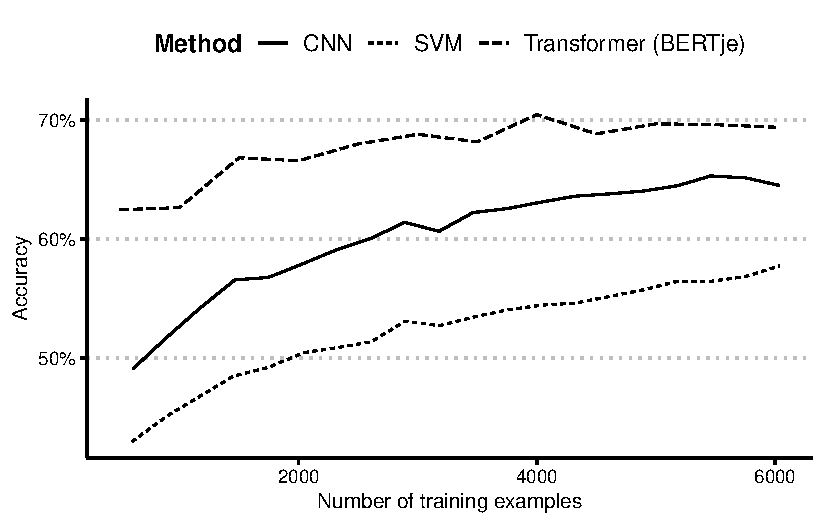
\includegraphics{grafzahl_sp_files/figure-pdf/fig-fig1-1.pdf}

}

\caption{\label{fig-fig1}Learning curve of machine learning algorithms}

\end{figure}

\hypertarget{step-5-explain-the-prediction}{%
\subsubsection{Step 5: Explain the
prediction}\label{step-5-explain-the-prediction}}

Unlike ``glass-box'' machine learning models (Dobbrick et al. 2021),
Transformer-based prediction models are ``black-box''. There are so many
parameters in Transformers (the BERT base model has 110 million
parameters) and this complexity makes each individual parameter of a
model not interpretable.

A reasonable compromise is to make the prediction \emph{explainable}
instead. Generating Local Interpretable Model-agnostic Explanations
(LIME) (Ribeiro, Singh, and Guestrin 2016; R implementation by Pedersen
and Benesty 2021) is a good way to explain how the model makes its
prediction. The gist of the method is to perturb the input text data by
deleting parts of the sentence. For example: the sentence ``I hate this
movie'' will be perturbed as ``I this movie'', ``I hate movie'', ``I
hate this'', ``I hate'' etc. These perturbed sentences are then feed
into the machine learning model to make predictions. The relationship
between what get deleted and the prediction is studied. The parts that
change the prediction a lot would be more \emph{causal} to the original
prediction.

With the trained model, we can explain the predictions made for the
following two Dutch headlines: \emph{``Dijsselbloem pessimistisch over
snelle stappen Grieken''} (Dijsselbloem {[}the Former Minister of
Finance of the Netherlands{]} pessimistic about rapid maneuvers from
Greeks) and \emph{``Aandelenbeurzen zetten koersopmars voort''} (Stock
markets continue to rise). Models trained with \texttt{grafzahl} support
the R package \texttt{lime} directly. One can get explanations using the
following code:

\begin{Shaded}
\begin{Highlighting}[]
\FunctionTok{require}\NormalTok{(lime)}
\NormalTok{sentences }\OtherTok{\textless{}{-}}
    \FunctionTok{c}\NormalTok{(}\StringTok{"Dijsselbloem pessimistisch over snelle stappen Grieken"}\NormalTok{,}
      \StringTok{"Aandelenbeurzen zetten koersopmars voort"}\NormalTok{)}
\NormalTok{explainer }\OtherTok{\textless{}{-}} \FunctionTok{lime}\NormalTok{(training\_corpus, model)}
\NormalTok{explanations }\OtherTok{\textless{}{-}} \FunctionTok{explain}\NormalTok{(sentences, explainer, }\AttributeTok{n\_labels =} \DecValTok{1}\NormalTok{,}
                        \AttributeTok{n\_features =} \DecValTok{3}\NormalTok{)}
\FunctionTok{plot\_text\_explanations}\NormalTok{(explanations)}
\end{Highlighting}
\end{Shaded}

\begin{figure}

{\centering 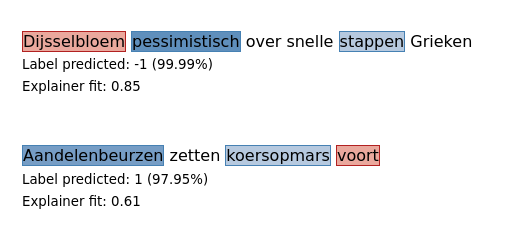
\includegraphics[width=3.43in,height=\textheight]{fig1.png}

}

\caption{\label{fig-fig2}Generating Local Interpretable Model-agnostic
Explanations (LIME) of two predictions from the trained Dutch sentiment
model}

\end{figure}

Figure~\ref{fig-fig2} shows that for the sentence \emph{``Dijsselbloem
pessimistisch over snelle stappen Grieken''} (classified as negative),
the tokens \emph{pessimistisch} and \emph{stappen} are making the
prediction towards the classified position (negative). But the token
\emph{Dijsselbloem} is making it away.

\hypertarget{non-germanic-example-amharic}{%
\section{Non-Germanic example:
Amharic}\label{non-germanic-example-amharic}}

I want to emphasize that \texttt{grafzahl} is not just another package
focusing only on English, or Germanic languages such as Dutch. Baden et
al. (2021) criticize this tendency.

Amharic is a Semitic language mainly spoken in Ethiopia and is in
general considered to be a ``low resource'' language. (Joshi et al.
2020) Only recently, the first news classification dataset called
``Amharic News Text classification Dataset'' is available (Azime and
Mohammed 2021). The dataset contains 50,706 news articles curated from
various Amharic websites. The original paper reports the baseline
out-of-sample accuracy of 62.2\% using Naive Bayes. The released data
also contains the training-and-test split \footnote{\url{https://huggingface.co/datasets/israel/Amharic-News-Text-classification-Dataset}}.
In this example, the AfriBERTa is used as the pretrained model (Ogueji,
Zhu, and Lin 2021). The AfriBERTa model was trained with a small corpus
of 11 African languages. Similar to the previous example, the default
settings of \texttt{grafzahl} are used.

\begin{Shaded}
\begin{Highlighting}[]
\NormalTok{input }\OtherTok{\textless{}{-}} \FunctionTok{get\_amharic\_data}\NormalTok{()}
\NormalTok{model }\OtherTok{\textless{}{-}} \FunctionTok{grafzahl}\NormalTok{(}\AttributeTok{x =}\NormalTok{ input}\SpecialCharTok{$}\NormalTok{training,}
                  \AttributeTok{y =} \StringTok{"category"}\NormalTok{,}
                  \AttributeTok{model\_name =} \StringTok{"castorini/afriberta\_base"}\NormalTok{)}

\DocumentationTok{\#\# Calculate the out{-}of{-}sample accuracy}

\NormalTok{preds }\OtherTok{\textless{}{-}} \FunctionTok{predict}\NormalTok{(model, }\AttributeTok{newdata =}\NormalTok{ input}\SpecialCharTok{$}\NormalTok{test)}
\NormalTok{caret}\SpecialCharTok{::}\FunctionTok{confusionMatrix}\NormalTok{(}\FunctionTok{table}\NormalTok{(preds, }\FunctionTok{docvars}\NormalTok{(input}\SpecialCharTok{$}\NormalTok{test,}
                                            \StringTok{"category"}\NormalTok{)))}
\end{Highlighting}
\end{Shaded}

\hypertarget{results}{%
\subsection{Results}\label{results}}

The final out-of-sample accuracy is 84.18\%, a solid improvement from
the baseline of 62.2\%.

\hypertarget{conclusion}{%
\section{Conclusion}\label{conclusion}}

This paper presents the R packages \texttt{grafzahl} and demonstrates
its applicability to communication research by replicating the
supervised machine learning part of published communication research.

\hypertarget{acknowledgments}{%
\section{Acknowledgments}\label{acknowledgments}}

I would like to thank 1) Jarvis Labs for providing discounted GPU cloud
service for the development of this package; 2) Pablo Barberá
(University of Southern California) and Wouter van Atteveldt (VU
Amsterdam) for allowing me to include their datasets in this package.

\hypertarget{references}{%
\section*{References}\label{references}}
\addcontentsline{toc}{section}{References}

\hypertarget{refs}{}
\begin{CSLReferences}{1}{0}
\leavevmode\vadjust pre{\hypertarget{ref-azime2021amharic}{}}%
Azime, Israel Abebe, and Nebil Mohammed. 2021. {``{An Amharic News Text
classification Dataset}.''} \emph{arXiv Preprint arXiv:2103.05639}.

\leavevmode\vadjust pre{\hypertarget{ref-baden:2021:TGC}{}}%
Baden, Christian, Christian Pipal, Martijn Schoonvelde, and Mariken A.
C. G van der Velden. 2021. {``Three Gaps in Computational Text Analysis
Methods for Social Sciences: A Research Agenda.''} \emph{Communication
Methods and Measures} 16 (1): 1--18.
\url{https://doi.org/10.1080/19312458.2021.2015574}.

\leavevmode\vadjust pre{\hypertarget{ref-quantedatextmodels}{}}%
Benoit, Kenneth, Kohei Watanabe, Haiyan Wang, Patrick O. Perry, Benjamin
Lauderdale, Johannes Gruber, and William Lowe. 2021.
\emph{Quanteda.textmodels: {Scaling Models and Classifiers for Textual
Data}}. \url{https://CRAN.R-project.org/package=quanteda.textmodels}.

\leavevmode\vadjust pre{\hypertarget{ref-ccoltekin2020corpus}{}}%
Çöltekin, Çağrı. 2020. {``{A corpus of Turkish offensive language on
social media}.''} In \emph{Proceedings of the 12th Language Resources
and Evaluation Conference}, 6174--84.

\leavevmode\vadjust pre{\hypertarget{ref-de2019bertje}{}}%
de Vries, Wietse, Andreas van Cranenburgh, Arianna Bisazza, Tommaso
Caselli, Gertjan van Noord, and Malvina Nissim. 2019. {``{Bertje: A
Dutch BERT model}.''} \emph{arXiv Preprint arXiv:1912.09582}.

\leavevmode\vadjust pre{\hypertarget{ref-dobbrick:2021:ETI}{}}%
Dobbrick, Timo, Julia Jakob, Chung-Hong Chan, and Hartmut Wessler. 2021.
{``Enhancing Theory-Informed Dictionary Approaches with {`Glass-Box'}
Machine Learning: The Case of Integrative Complexity in Social Media
Comments.''} \emph{Communication Methods and Measures}, November, 1--18.
\url{https://doi.org/10.1080/19312458.2021.1999913}.

\leavevmode\vadjust pre{\hypertarget{ref-joshi2020state}{}}%
Joshi, Pratik, Sebastin Santy, Amar Budhiraja, Kalika Bali, and Monojit
Choudhury. 2020. {``The State and Fate of Linguistic Diversity and
Inclusion in the NLP World.''} \emph{arXiv Preprint arXiv:2004.09095}.

\leavevmode\vadjust pre{\hypertarget{ref-kuhn:2008:BPM}{}}%
Kuhn, Max. 2008. {``Building Predictive Models in {R} Using the Caret
Package.''} \emph{Journal of Statistical Software} 28 (5).
\url{https://doi.org/10.18637/jss.v028.i05}.

\leavevmode\vadjust pre{\hypertarget{ref-ogueji2021small}{}}%
Ogueji, Kelechi, Yuxin Zhu, and Jimmy Lin. 2021. {``Small Data? No
Problem! Exploring the Viability of Pretrained Multilingual Language
Models for Low-Resourced Languages.''} In \emph{Proceedings of the 1st
Workshop on Multilingual Representation Learning}, 116--26.

\leavevmode\vadjust pre{\hypertarget{ref-lime}{}}%
Pedersen, Thomas Lin, and Michaël Benesty. 2021. \emph{Lime: Local
Interpretable Model-Agnostic Explanations}.
\url{https://CRAN.R-project.org/package=lime}.

\leavevmode\vadjust pre{\hypertarget{ref-simpletransformers}{}}%
Rajapakse, Thilina. 2022. \emph{{Simple Transformers}}.
\url{https://simpletransformers.ai/}.

\leavevmode\vadjust pre{\hypertarget{ref-ribeiro2016should}{}}%
Ribeiro, Marco Tulio, Sameer Singh, and Carlos Guestrin. 2016. {``"Why
Should i Trust You?" Explaining the Predictions of Any Classifier.''} In
\emph{Proceedings of the 22nd ACM SIGKDD International Conference on
Knowledge Discovery and Data Mining}, 1135--44.

\leavevmode\vadjust pre{\hypertarget{ref-theocharis:2020:DPI}{}}%
Theocharis, Yannis, Pablo Barberá, Zoltán Fazekas, and Sebastian Adrian
Popa. 2020. {``The Dynamics of Political Incivility on Twitter.''}
\emph{SAGE Open} 10 (2): 215824402091944.
\url{https://doi.org/10.1177/2158244020919447}.

\leavevmode\vadjust pre{\hypertarget{ref-reticulate}{}}%
Ushey, Kevin, JJ Allaire, and Yuan Tang. 2022. \emph{{reticulate:
Interface to 'Python'}}.
\url{https://CRAN.R-project.org/package=reticulate}.

\leavevmode\vadjust pre{\hypertarget{ref-atteveldt:2021:VSA}{}}%
Van Atteveldt, Wouter, Mariken A. C. G. Van der Velden, and Mark Boukes.
2021. {``The Validity of Sentiment Analysis:comparing Manual Annotation,
Crowd-Coding, Dictionary Approaches, and Machine Learning Algorithms.''}
\emph{Communication Methods and Measures}, January, 1--20.
\url{https://doi.org/10.1080/19312458.2020.1869198}.

\leavevmode\vadjust pre{\hypertarget{ref-wolf-etal-2020-transformers}{}}%
Wolf, Thomas, Lysandre Debut, Victor Sanh, Julien Chaumond, Clement
Delangue, Anthony Moi, Pierric Cistac, et al. 2020. {``Transformers:
State-of-the-Art Natural Language Processing.''} In \emph{Proceedings of
the 2020 Conference on Empirical Methods in Natural Language Processing:
System Demonstrations}, 38--45. Online: Association for Computational
Linguistics. \url{https://www.aclweb.org/anthology/2020.emnlp-demos.6}.

\end{CSLReferences}



\end{document}
